%%%%%%%%%%%%%%%%%%%%%%%%%%%%%%%%%%%%%%%%%%%%%%%%%%%%%%%%%%%%%%%%%%%%%%%%%%%%%%%%%%%%%%%%%%%%%%%
%                                     TRANSFER LEARNING                                       %
%%%%%%%%%%%%%%%%%%%%%%%%%%%%%%%%%%%%%%%%%%%%%%%%%%%%%%%%%%%%%%%%%%%%%%%%%%%%%%%%%%%%%%%%%%%%%%%
\chapter{Transfer Learning}
\label{chap:transfer}

\begin{chapabstract}
After a brief tour of the landscape of transfer learning methods in Section~\ref{sec:transfer}, we introduce the problem of kidney segmentation in 3D ultrasound images across two populations: healthy adults and sick children (Section~\ref{sec:kidney}), which will be the main application of the methods proposed. Using standard transfer learning methods as our baseline in Section~\ref{sec:kidney_baseline} was insufficient for our problem and led us to develop a new transfer learning method presented in Section~\ref{sec:transfo}. That method is based on predicting transformations to be applied to images during inference. We wrap up the chapter with a comparison of the tested methods and a discussion of the results in Section~\ref{sec:kidney_res} and a conclusion in Section~\ref{sec:transfer_conclusion}.
\end{chapabstract}

\vspace{1cm}

{   
    \setstretch{1.0}
    \minitoc
}
\newpage

%%%%%%%%%%%%%%%%%%%%%%%%%%%%%%%%%%%%%%%%%%%%%%%%%%%%%%%%%%%%%%%%%%%%%%%%%%%%%%%%%%%%%%%%%%%%%%%
\section{The many different faces of transfer learning}
\label{sec:transfer}

Transfer learning is the idea of re-using knowledge learned in one situation for another situation. This makes intuitive sense in many frequently encountered cases. To take examples from the medical field, a model trained on the detection of a specific disease in a specific imaging protocol should have learned something about these images that could be used for the detection of another disease. Those images have common properties like the intensity of organs and bones that computer vision models learn and use. Transfer learning aim to avoid re-learning those properties but instead transfer them from one model to the other. Models may also learn other kinds of knowledge, such as the anatomy of the human body. Organs do not change shape or location from one imaging protocol to the other, and models may learn and use this information.

But to be useful, transfer learning must be faster or more convenient than simply training a model from scratch. In the medical field in particular, the acquisition of data is costly and time-consuming, and labeling or segmenting the acquired data to build a training database even more so. It is very common to have only a handful of patients from a particular population. That scarcity of data may make some tasks unsolvable by themselves, but pooling together every available bit of data may allow solving them. 

\begin{figure}[htb]
    \centering
	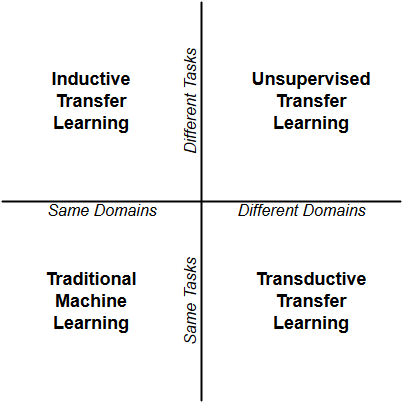
\includegraphics[width=0.5\textwidth]{img_transfer/transfer_types.png}
    \caption[Transfer learning categories]{Transfer learning can be divided into four categories depending on how the domains and the tasks are related.}
    \label{fig:transfer_types}
\end{figure}

Following the notation of~\textcite{pan2010TNDE}, we define the \textit{domain} as a feature space $\mathcal{X}$ and a probability distribution $P\left( \mathrm{X} \right)$ such that $\mathrm{X} = \{ x_1, \cdots, x_n \} \in \mathcal{X}$. A \textit{task} is composed of a label space $\mathcal{Y}$ and an objective predictive function $f$ which is learned from the training data (i.e. pairs of $\{ x_i, y_i \}$ where $x_i \in \mathcal{X}$ and $y_i \in \mathcal{Y}$). The transfer is done from a \textit{source} domain and task to a \textit{target} domain and task. These notions form the two axes according to which transfer learning methods are divided. How are the source and target domains related, and how are the source and target tasks related? These axes result in four different problems as shown in Figure~\ref{fig:transfer_types}. 

Inductive transfer learning is the category of problems where the source and target domains are identical, while the source and target tasks are different, but related. An example of such a problem would be an image database where the source task is to detect the presence or absence of particular objects and the target task is to locate those objects in the image. Transductive transfer learning is the category where the source and target domains are different but related, while the source and target tasks are identical. An example that we introduce in Section~\ref{sec:kidney} is the segmentation of the kidney in 3D ultrasound images, where the source domain is composed of healthy adults and the target domain is composed of sick children. Unsupervised transfer learning happens when both the domains and the tasks are different. In this setting, labels are unavailable for both source and target. In all three cases, transfer of knowledge is possible by exploiting the nature of the differences between the domains and the tasks.

In this section we briefly present these three kinds of transfer learning. Then Section~\ref{ssec:deep_transfer} focuses on transfer learning in the context of deep learning.

If both the domains and the tasks are identical, this is simply standard machine learning and not transfer learning.

%%%%%%%%%%%%%%%%%%%
\subsection{Inductive Transfer Learning}
\label{ssec:inductive}

In this setting, the source and target tasks are different, while the source and target domains stay the same. Many approaches have been explored in this setting. An extension of the AdaBoost algorithm, TrAdaBoost (\textcite{dai2007ICML}), assumes that data in the source and target domains share features and labels but have different distributions, in order to propose an iterative reweighting of the source domain data during training. 

Learning a low-dimensional representation of the data that is shared across tasks is an idea explored in a supervised fashion (\textcite{argyriou2006NIPS},~\textcite{lee2007ICML}) and in an unsupervised fashion (\textcite{raina2007ICML}).

It is also possible to transfer parameters or hyper-parameters of various models. \textcite{lawrence2004ICML} proposed to learn kernel parameters for Gaussian processes across tasks,~\textcite{evgeniou2004} developed a regularization framework for sharing parameters of SVMs. \textcite{gao2008} built an ensemble learning framework where the weights of each model are assigned dynamically for each sample in the target domain.

%%%%%%%%%%%%%%%%%%%
\subsection{Transductive Transfer Learning}
\label{ssec:transductive}

Transductive transfer learning (\textcite{arnold2007}), also called domain adaptation, focuses on solving the same task across different domains. The difficulty comes when little data is available in the target domain, or when labels are unavailable or sparse for the target domain. A lot of work has been done on how to relate the unlabeled target data with the labeled data through the loss of the model (\textcite{arnold2007})) or in which proportion they should be mixed during training (\textcite{crammer2008JMLR},~\textcite{ben-david2010}).

When the model learns simultaneously on the different domains, this is multi-domain learning (\textcite{daume2007},~\textcite{joshi2013}).

%%%%%%%%%%%%%%%%%%%
\subsection{Unsupervised Transfer Learning}
\label{ssec:unsupervised}

There has been relatively little work in this setting.~\textcite{dai2008ICML} proposed a \textit{self-taught clustering} algorithm which aims to cluster a small unlabeled target dataset at the same time as a big unlabeled source dataset. By learning a common feature space, clustering on the target dataset is improved.

\textcite{chang2018} developed a method to learn a bank of multi-scale convolutional filters from a large unlabeled source dataset and a small target dataset, which can then be used in a convolutional neural network to solve classification tasks. Only the construction of the filters bank is done without labels. Applications on various biomedical tasks show a clear improvement in performance over using only the target dataset.

%%%%%%%%%%%%%%%%%%%
\subsection{Transfer Learning and Deep Learning}
\label{ssec:deep_transfer}

One method has become the \textit{de facto} face of transfer learning for deep neural networks, due to its simplicity and versatility: fine-tuning (\textcite{hinton2006},~\textcite{bengio2007NIPS}). The idea is that the features learned by a neural network are generic enough, so that it becomes interesting to re-use them on a different domain, for a different task, or both. No modifications to the architecture are done. The only difference is that the weights of the network are not initialized randomly, but set to the final weights learned on the source domain.

\begin{figure}[htbp]
    \centering
	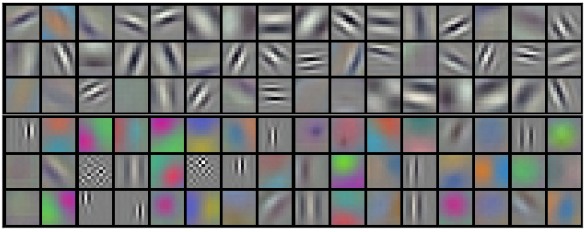
\includegraphics[width=\textwidth]{img_transfer/alexnet_gabor}
    \caption[Gabor filters learned by AlexNet]{The first convolutional layer of AlexNet learned many filters very similar to Gabor filters. (Source:~\textcite{krizhevsky2012NIPS})}
    \label{fig:alexnet_gabor}
\end{figure}

It is not always necessary, or even a good idea, to re-train the whole network. If the target dataset is too small, full fine-tuning risks overfitting. But then, which layers should be fine-tuned? Lower layers tend to be more generic, while higher layers tend to be specialized to the task (\textcite{yosinski2014NIPS}), suggesting that it would be better to fine-tune only the last $n$ layers of the network. As illustrated in Figure~\ref{fig:alexnet_gabor}, the AlexNet architecture trained on ImageNet learns filters very similar to Gabor filters in its first convolutional layer, showing their genericity. An additional advantage is that it is faster as there is no need to back-propagate to the lower layers. The exact value of $n$ is entirely problem-specific, the closer the domains and the tasks are, the less layers need to be fine-tuned.

Moreover the source dataset does not need to be closely related to the target dataset. A network trained for classification on the ImageNet dataset (\textcite{imagenet}) can be fine-tuned on other natural images dataset for classification or even detection and improve the results over training from scratch (\textcite{oquab2014CVPR},~\textcite{razavian2014CVPR}).

An alternative to fine-tuning is feature extraction (\textcite{donahue14PMLR},~\textcite{sermanet2014ICLR}). It is similar to fine-tuning in that it uses the fact that the features learned by the lower layers of a neural network are fairly generic. But instead of modifying the higher layers of the network, here they are discarded and the output of the lower layers are used as features for a completely different model, not necessarily a neural network (see Figure~\ref{fig:feature_extraction}). Features extracted from natural images have been shown to be useful to medical images (\textcite{shin2016},~\textcite{bar2015ISBI},~\textcite{vanginneken2015ISBI}).

\begin{figure}[htbp]
    \centering
	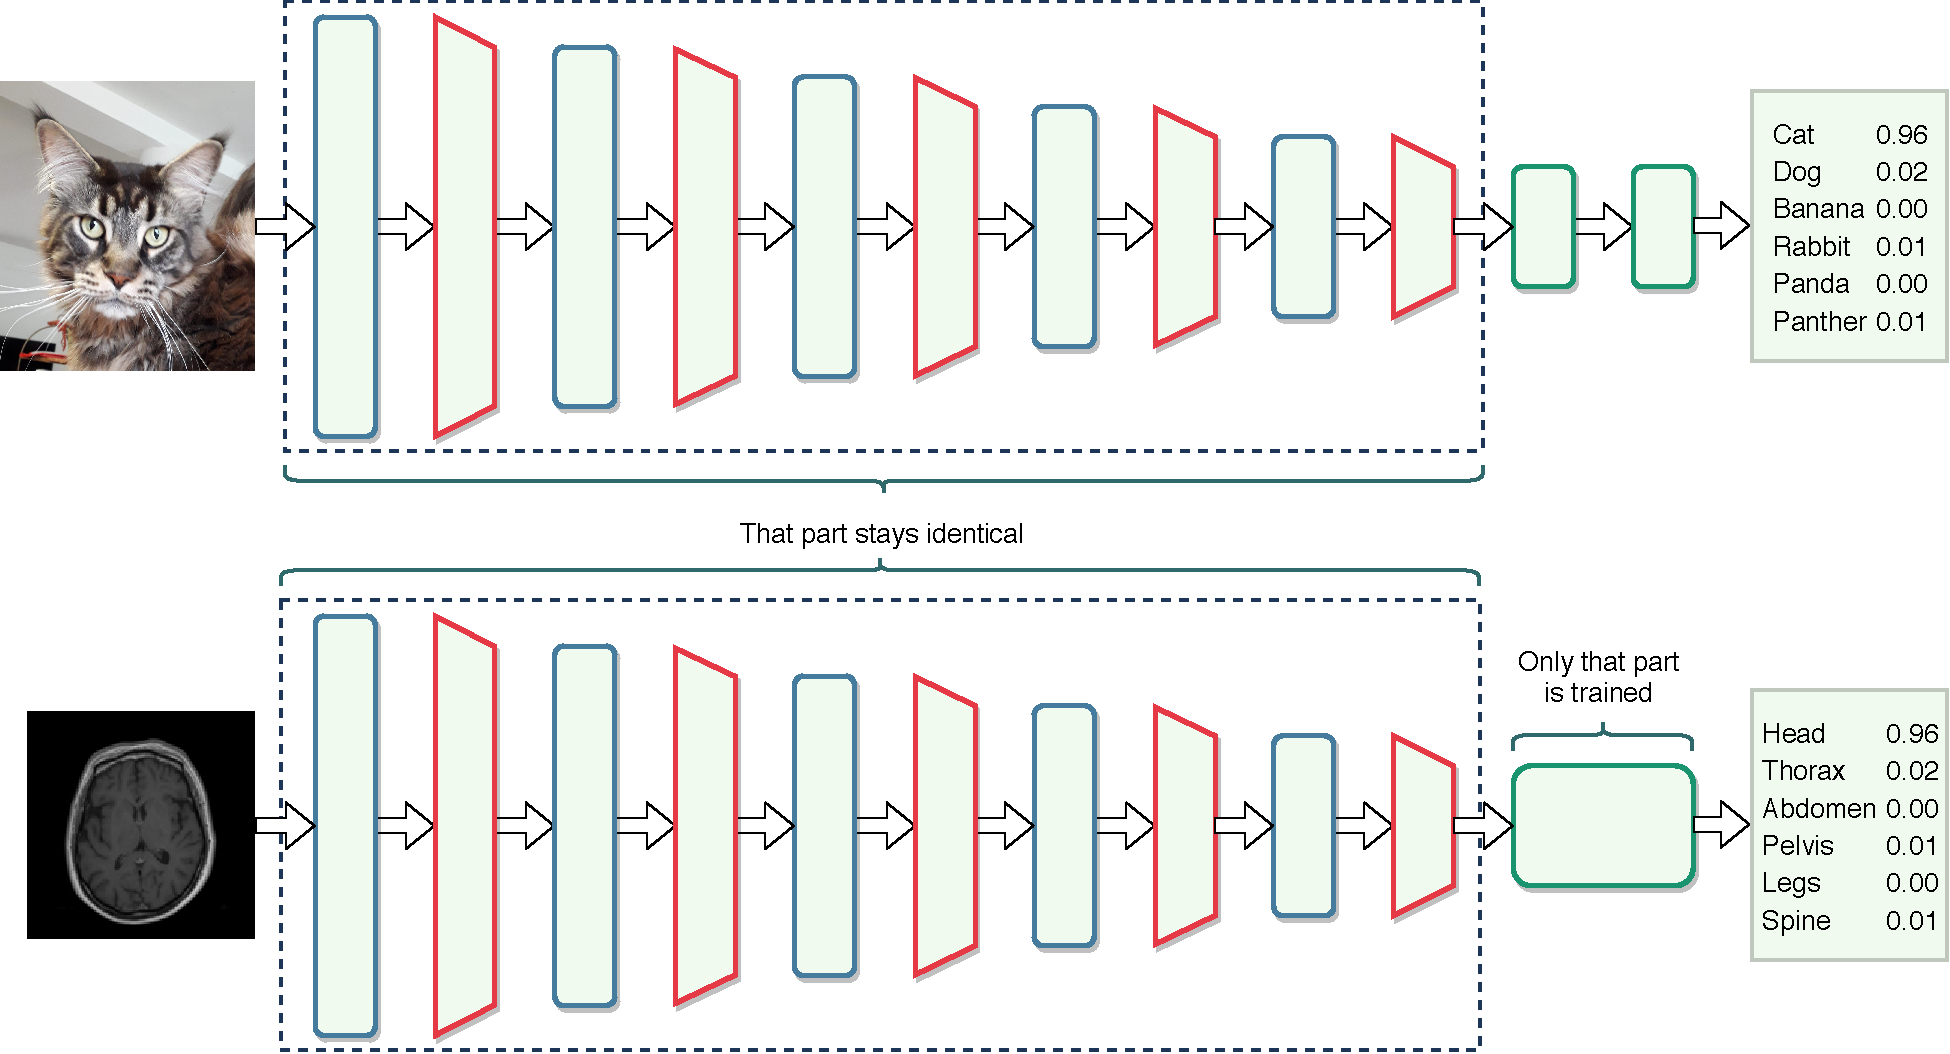
\includegraphics[width=\textwidth]{img_transfer/feature_extraction}
    \caption[Feature Extraction]{Feature Extraction. The network at the top is trained on natural images. It can be reused on medical images by extracting the features at a given layer of the network and using them as the input of a new model.}
    \label{fig:feature_extraction}
\end{figure}

Autoencoders (\textcite{ballard1987},~\textcite{bengio2007NIPS}) are neural networks learned in an unsupervised manner. The goal of the network is to reconstruct its input from a compressed representation of the data that it will learn. The first part of the network progressively compresses the input while the second part decompresses it. This first part can then be used as a pre-trained network for other datasets and tasks (\textcite{bengio2007NIPS},~\textcite{vincent2008ICML},~\textcite{erhan2010JMLR}). The representation learned by the autoencoder can also be used as the features of another model, which is helpful even for distant domains such as natural images and MR images (\textcite{gupta2013ICML}). More generally, unsupervised pre-training on natural images has successfully been used to improve results on medical imaging tasks (\textcite{schlegl2014MICCAI},~\textcite{hofmanninger2015CVPR}).

The methods discussed so far assume a sequence of actions. First a source task is solved on a source domain, and then a target task is solved on a target domain. But if the different tasks are defined from the start, it makes sense to solve them simultaneously. This is the idea of multitask training (\textcite{caruana1995NIPS},~\textcite{caruana1997},~\textcite{collobert2008ICML}). It consistently gives better results on both tasks than sequential transfer methods. 

Likewise, when solving a task on different domains accessible from the start, it makes sense to use the different domains at the same time. The simplest method is to train the network on the union of the different domains, but this does not work well when one domain is a lot bigger than the other. Weighting each sample according to the number of samples of each domain (\textcite{daume2007}) or balancing batches across domains during training (\textcite{buda2017}) fixes this problem. More complex multi-domain training methods exist, such as~\textcite{nam2016CVPR} where the network learns domain-specific convolutional layers.


%Finetuning across domains and tasks~\textcite{tzeng2015ICCV}.


%GAN DA~\textcite{kamnitsas2017IPMI}

%%%%%%%%%%%%%%%%%%%%%%%%%%%%%%%%%%%%%%%%%%%%%%%%%%%%%%%%%%%%%%%%%%%%%%%%%%%%%%%%%%%%%%%%%%%%%%%
\section{Kidney Segmentation in 3D Ultrasound}
\label{sec:kidney}

%%%%%%%%%%%%%%%%%%%%%%%%%%%%%%%%%%
\subsection{Introduction}

%A common (and often disappointing) scenario in clinical settings is to expect an algorithm, built on a specific class of medical images, to succeed at the same task on data judged similar by the clinician. Focusing on the particular class of deep learning-based methods, we propose a transfer approach to, if not instantly, quickly satisfy this expectation. We work under the assumption that no access to the original training database is possible, as it is frequently the case in practice. 

The clinical problem motivating this work is the kidney capsule segmentation in 3D ultrasound data from potentially ill children. These images have a high amount of noise, strong dependency on the operator, and important organ shape variability induced by subjects age and degree of illness. Moreover we have limited access to such volumes. In contrast, a much larger database of ultrasound kidney volumes of healthy adults is available, from which we build a successful segmenting deep network. We aim to transfer the knowledge (anatomy, US signal, ...) captured by this network to the pediatric data. 

This work has contributions in both the clinical and technical domains: (i) a deep learning based algorithm for kidney capsule segmentation in 3D ultrasound data (Section~\ref{sec:kidney_baseline}), and (ii) a new approach to perform domain adaptation of a pre-trained neural network (Section~\ref{sec:transfo}). In addition we present experiments comparing different transfer methods according to performance, training time and added complexity to determine the trade-offs of each method (Section~\ref{sec:kidney_res}), and discuss their results, examining the segmentation errors to suggest potential improvements.

%%%%%%%%%%%%%%%%%%%%%%%%%%%%%%%%%%
\subsection{Related Work}

%\subsubsection{Kidney segmentation in 3D ultrasound data}

Despite the clinical potential of 3D kidney ultrasounds, both the number of publications and the data used within are relatively small. Moreover, to the best our knowledge, deep learning techniques have not yet been applied.~\textcite{cerrolaza2014ISBI} and~\textcite{marsousi2017} have addressed the capsule segmentation problem in 3D pediatric data using active shape models and for real-time segmentation using implicit deformable models, respectively. 
%In fact, we have not found any paper using deep learning for the segmentation of the kidney in 3D ultrasound.

Nevertheless, deep learning techniques have been applied by~\textcite{ravishankar2017MICCAI} to 2D ultrasound kidney images. Their approach is compelling since they manage to combine deep learning and shape priors by using two networks, first a U-Net for the segmentation, then a convolutional auto-encoder as a shape prior used for regularization.

The baseline to our work (Section~\ref{ssec:unet}) is the well-known deep learning architecture ``U-Net'' (\textcite{ronneberger2015MICCAI}) and its 3D version (\textcite{cicek2016MICCAI}). 

%DeepMedic is another framework developed for the segmentation of lesions in 3D MR brain images by Kamnitsas \textit{et al.}~\cite{kamnitsas_2017}. The segmentation is done in two parts, first the image go through a 3D convolutional neural network that outputs a segmentation map, which is then refined by a 3D conditional random field. Additionally, the CNN takes as input the image at normal resolution and a down-sampled version in order to incorporate multi-scale features.

%%%%%%%%%%%%%%%%%%%%%%%%%%%%%%%%%%
\subsection{Dataset}
\label{ssec:data}

\begin{figure}[htbp]
    \centering
	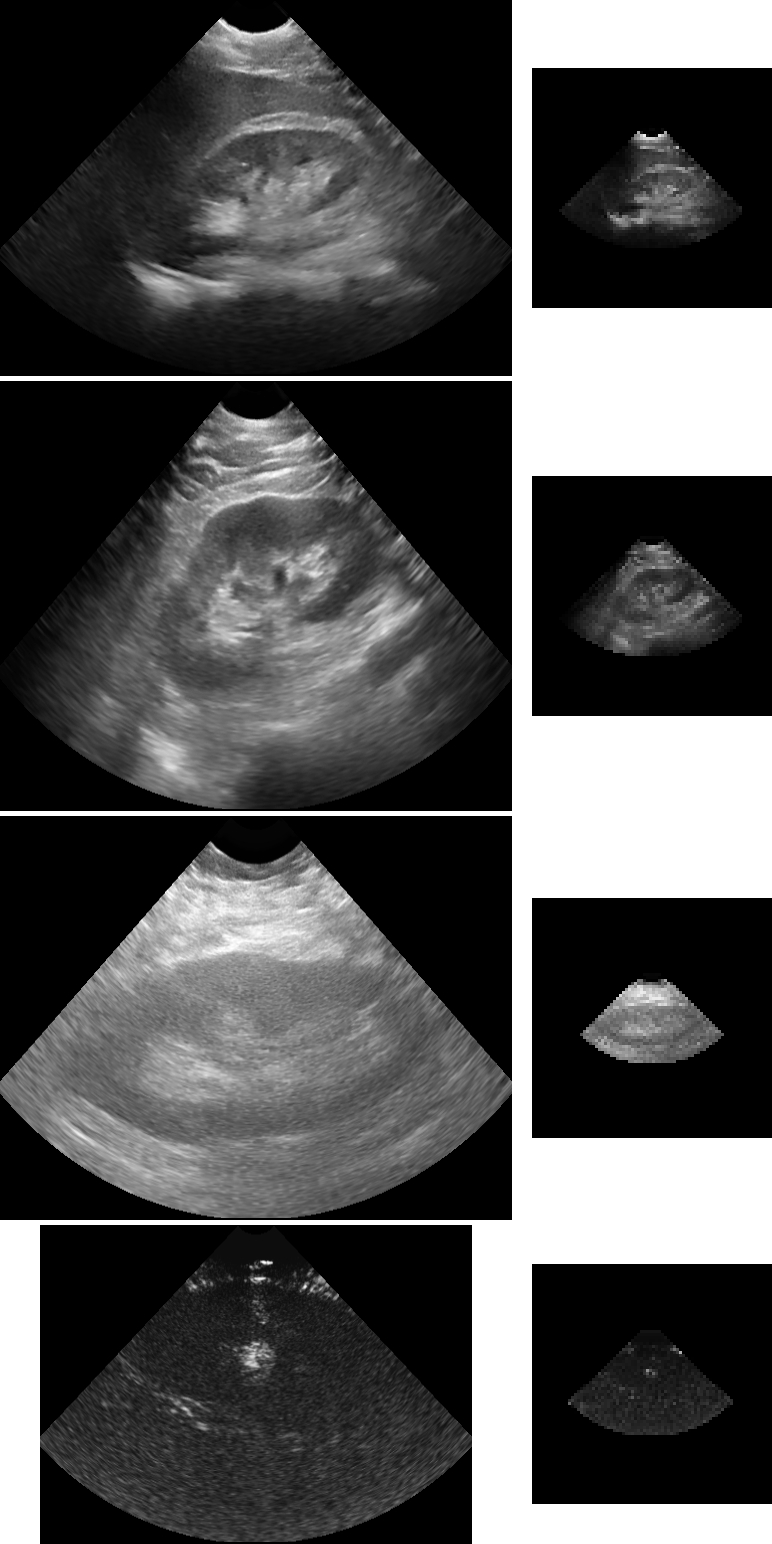
\includegraphics[width=0.67\textwidth]{img_transfer/adults_prep}
    \caption{Healthy adults kidneys before and after pre-processing.}
    \label{fig:adults_prep}
\end{figure}

\begin{figure}[htbp]
    \centering
	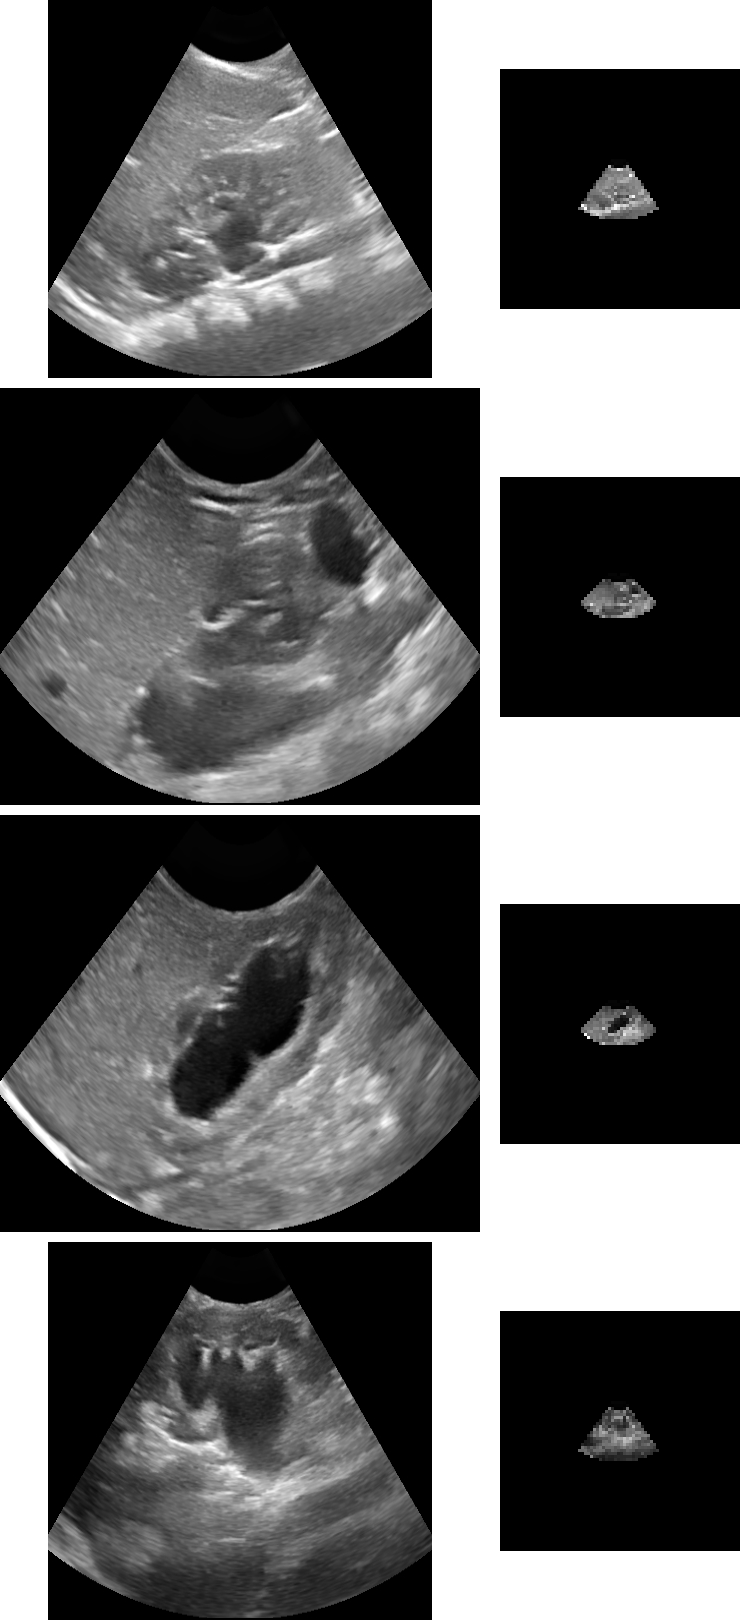
\includegraphics[width=0.6\textwidth]{img_transfer/children_prep}
    \caption{Sick children kidneys before and after pre-processing.}
    \label{fig:children_prep}
\end{figure}

The ultrasound volumes in our study come from several clinical sites around the world. As a result, there is a high variability in the quality of the images, which translates into various amounts of noise and shadow artifacts as can be seen in Figure~\ref{fig:adults_prep}. 

We have a total of 503 healthy adults images, and 64 children (aged between 6 months and 15 years), of which about $30 \%$ have hydronephrosis in various stages. The database was split into $80 \%$ of the images used for training, the rest for testing.

The volumes we give to the network have been down-sampled to a resolution of $4 \times 4 \times 4$ mm$^3$, and centered in a $80 \times 80 \times 80$ voxels cube. The size in voxels was chosen in order to fit the network and a volume on a single NVIDIA TITAN GPU. The resolution was chosen so that each volume would fit entirely in the cube. We show images before and after pre-processing in Figure~\ref{fig:adults_prep} for the adults and Figure~\ref{fig:children_prep} for the children.
%Because we are not segmenting fine structures but only the kidneys, a smaller resolution is not vital.

%%%%%%%%%%%%%%%%%%%%%%%%%%%%%%%%%%%%%%%%%%%%%%%%%%%%%%%%%%%%%%%%%%%%%%%%%%%%%%%%%%%%%%%%%%%%%%%
\section{Baseline}
\label{sec:kidney_baseline}

%%%%%%%%%%%%%%%%%%%%%%%%%
\subsection{3D U-Net}
\label{ssec:unet}

\begin{figure}[htb]
    \centering
	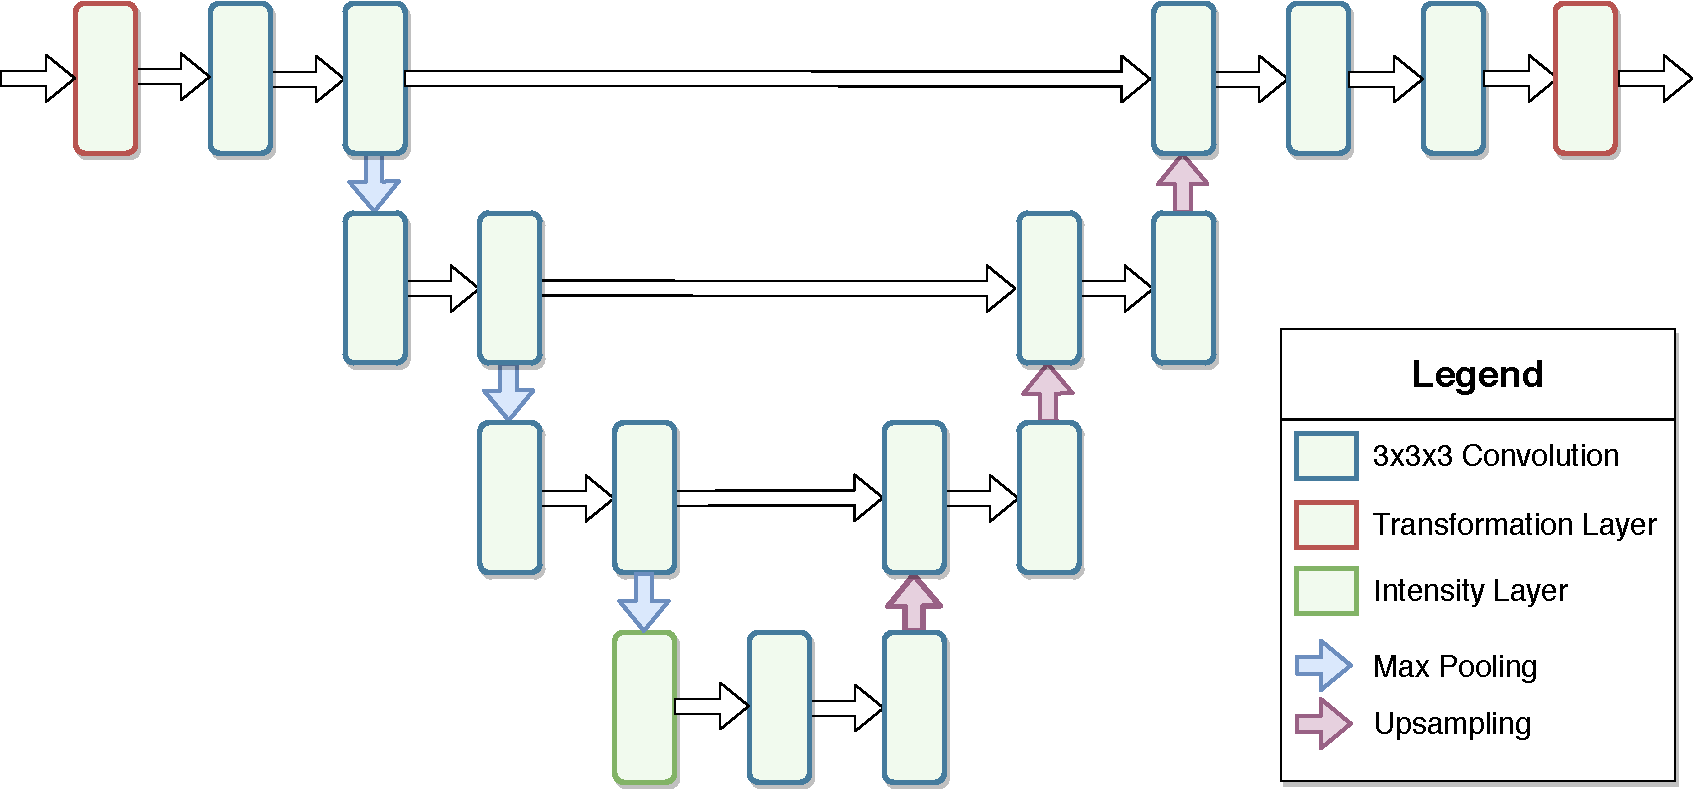
\includegraphics[width=\textwidth]{img_transfer/UNet}
    \caption{U-Net structure with our added transformation and intensity layers.}
    \label{fig:unet}
\end{figure}

The 3D extension (\textcite{cicek2016MICCAI}) of the U-Net (\textcite{ronneberger2015MICCAI}) architecture is our starting point. Its symmetrical structure alternates convolutional layers with down-sampling layers on one side and convolutional layers with up-sampling layers on the other (see Figure~\ref{fig:unet}). At each level, down-sampled feature maps are concatenated to up-sampled ones to give multi-scale information to the network. In our adaptation of this architecture we replace the weighted softmax loss by a Dice-based loss, more adapted to our segmentation task, which is defined as follow:

\begin{equation}
    DICE \left( Y, \hat{Y} \right) = \frac{2 |Y \cap \hat{Y}|}{|Y| + |\hat{Y}|}
\end{equation}

where $Y$ is the ground truth segmentation and $\hat{Y}$ is the predicted segmentation. The Dice varies between $0$ and $1$, where $0$ means the prediction and the ground truth are disjoint and $1$ means a perfect prediction.

Moreover, introducing Spatial Dropout (\textcite{tompson2015CVPR}) after each convolution-sampling block proved to significantly improve our results by preventing over-fitting. Whereas standard Dropout (\textcite{srivastava2014}) randomly sets pixels in the feature maps at zero, Spatial Dropout randomly sets filters at zero, making it more relevant for convolutional layers.

%%%%%%%%%%%%%%%%%%%%%%%%%
\subsection{Training the baseline}
\label{ssec:training_baseline}

We used Keras (\textcite{chollet2015keras}) with the Tensorflow backend (\textcite{tensorflow2015}). We performed each experiment on five seeds, which impacts both the separation of the data set into training and test sets, and the initialization of the weights of the networks.

Three models are used as baseline: one trained on adults kidneys only, which will also be used for transfer, one trained on children only, and one trained on both, with oversampling of the children to balance each set. Oversampling is a way of dealing with class imbalance (\textcite{buda2017}) and consists in balancing each epoch to have as many adults as children by drawing each children multiple times.

These baseline models allow us to judge the quality of each transfer method. A good transfer method should perform better (or close to) on the children kidneys than the children only network, while staying close to the performance of the adults only network on the adults. The joint model represents the ideal performance we can hope for on adults and children. Results are displayed in Table~\ref{table:results}, and illustrated in Figure~\ref{fig:mseg}.

%%%%%%%%%%%%%%%%%%%%%%%%%
\subsection{Fine-tuning}
\label{ssec:baseline_finetune}

The adult baseline network is fine-tuned on the children dataset, resulting in an important drop of performance on the adults and a comparable improvement on the children (see Table~\ref{table:results}). This is obtained by fine-tuning the whole network. 

\begin{figure}[htbp]
    \centering
	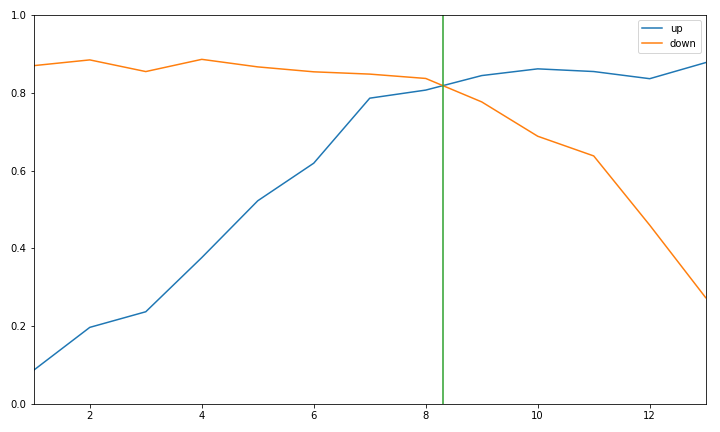
\includegraphics[width=0.7\textwidth]{img_transfer/partial_transfer}
    \caption[Partial fine-tuning]{Partial fine-tuning. The $x$ axis is the index of the layer and the y axis the Dice index. In blue, all the layers up to $x$ are fine-tuned. In orange, all the layers after $x$ are fine-tuned.}
    \label{fig:partial_transfer}
\end{figure}

It is however unnecessary as we show below. Fine-tuning only the last 7 convolutional layers of the network or the first 8 is enough to obtain the same results. This corresponds to all the layers before or after the first upsampling layer. Between the two options, fine-tuning the last layers is faster since there is no need to back-propagate to the early layers of the network.

%%%%%%%%%%%%%%%%%%%%%%%%%%%%%%%%%%%%%%%%%%%%%%%%%%%%%%%%%%%%%%%%%%%%%%%%%%%%%%%%%%%%%%%%%%%%%%%
\section{Transformation Layers}
\label{sec:transfo}

For our need, it is not enough to obtain good performance on the target dataset. We placed ourselves in a context where the transfer is done at a later time than the original training and the source dataset is not available anymore, but the network must still be able to segment those images. Because of the performance drop on the source dataset of the fine-tuning method, we must use something else.

Here we propose to introduce \textit{transfer} layers within the original model in order to adapt feature maps to the new dataset. We expect these layers to selectively adapt the network to children data while maintaining the network performance on adults.

%We selected six emplacements for adding layers: before the max-pooling and after the up-sampling, as shown in green in Figures ~\ref{fig:unet} and ~\ref{fig:block}. As each additional layer adds parameters and training time, but potentially allows for more capacity, we explored various combinations of emplacements to find the optimal trade-off. Each transfer block must have the same output size as its input to properly connect with the adjacent layer.

%As there is no obvious shape for the transfer layers, we designed a number of variations with different properties. The simplest was a single convolutional layer of $1 \times 1 \times 1$ filters. As $1 \times 1 \times 1$ convolutional layers do not capture locally spatial information, we also tested $3 \times 3 \times 3$ filters with the inconvenient of adding a high number of parameters (because we cannot reduce the number of filters). To solve this issue we used the following block: one $1 \times 1 \times 1$ convolutional layer with less filters to reduce dimensionality, followed by a max-pooling and a $3 \times 3 \times 3$ convolutional layer, then up-sampling and one last $1 \times 1 \times 1$ convolutional layer to recover the expected dimensionality. 
%One variant we tried was to make those layers residual. The intuition is that because the adults and the children are not so different, it might be easier to learn a correction of the feature maps rather than transform them directly.

When inserting new layers, it might be tempting to simply use standard convolutional layers. The problem is that as the parameters of these layers are fixed once the training is done, the same convolutions will be applied to all images and feature maps. Those new convolutions will heavily degrade performance on images from the original distribution. %It is also not obvious where to put those new layers. 

We tested many variations of position and shape of those additional convolutional layers. The combination with the highest performance was to add a convolutional layer after each downsampling or upsampling layers, i.e. 6 new layers with filters of size $3 \times 3 \times 3$. This was enough to barely reach the performance of the fine-tuning method, while taking longer and adding 23 millions parameters to the network. 

We instead propose to predict parameters during inference for each image. Images from the source distribution will have parameters predicted close to the identity transform, while images from the target distribution can be transformed to be more similar to the source distribution. We introduce two kinds of transfer layers with different goals.

%One crucial point when adding a layer is to initialize its weights such that the layer is an identity layer at first, meaning that the output is equal to the input. Initializing weights randomly completely destroys the performance and the learning process is unable to recover.

%%%%%%%%%%%%%%%%%%%
\subsection{Geometric Transformation Layer}
\label{ssec:geo_transfo}

Working within the same image modality, we propose to use geometric transformations as transfer layers in order to effectively transfer information between our datasets (adults to children). This is similar to the Spatial Transformer proposed by~\textcite{jaderberg2015NIPS}, but instead of predicting directly the parameters of the transformation, we predict the amount of translation, rotation and scaling along each axis, i.e. nine parameters in total. These parameters are then used by the transformation layer to geometrically modify its input using tri-linear interpolation. There is no attention mechanism.

We place this layer at the entrance of the network and perform the inverse transformation at the output of the network as shown in Figure~\ref{fig:unet}. The transformation can be seen as a projection on the adults space, and therefore we need to project back on the children space at some point. The prediction of the parameters is done with a 3-layers convolutional network taking the image as input.

%%%%%%%%%%%%%%%%%%%
\subsection{Intensity Layer}
\label{ssec:intensity_transfo}

\begin{figure}[htb]
	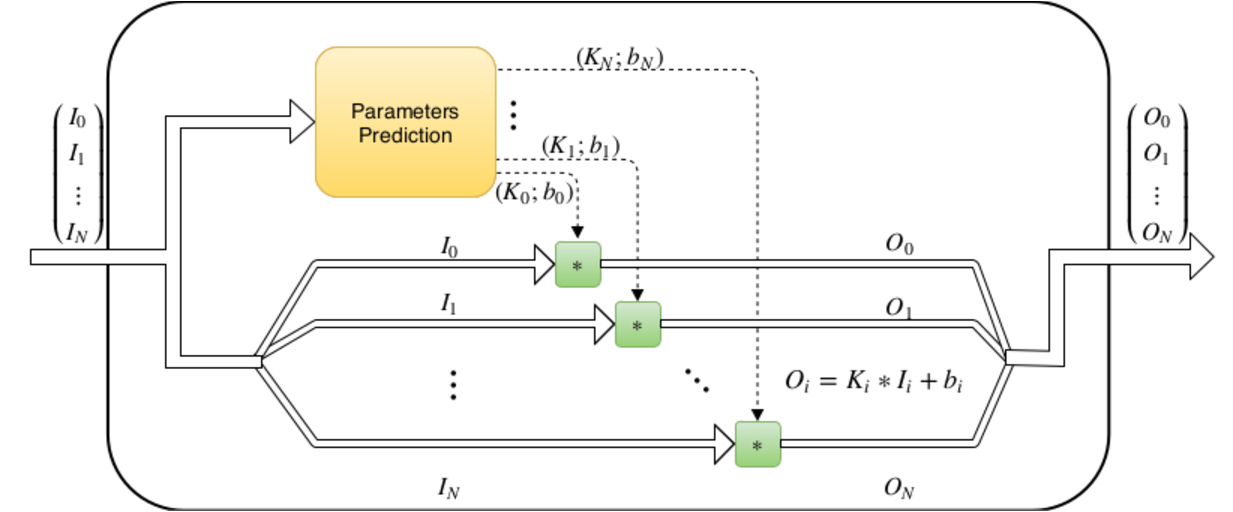
\includegraphics[width=\textwidth]{img_transfer/Intensity_Block}
    \caption[Intensity Layer]{Intensity Layer. ``Parameters Prediction'' can be any model, in our case it is a 3-layers ConvNet.}
    \label{fig:block}
\end{figure}

A geometric transformation is not enough to express the differences between the source and target datasets. We therefore propose to predict an intensity transformation, implemented as a $1 \times 1 \times 1$ convolution applied to each feature map, shown in Figure~\ref{fig:block}. Noting $I = \{ I_1, \cdots, I_n \}$ the input feature maps and $\theta$ the weights of the parameters prediction component, the exact transformation applied to each feature map $I_i$ is:
\begin{equation*}
O \left( I_i \right) = K_i \left( I; \theta \right) * I_i + b_i \left( I; \theta \right)
\end{equation*}
where $K_i \left( I; \theta \right)$ and $b_i \left( I; \theta \right)$ are the predicted parameters. In the end, two parameters have to be predicted for each feature map. Experiments showed that this layer works best when placed at the lowest level of the U-Net (see Figure~\ref{fig:unet}).

%%%%%%%%%%%%%%%%%%%%%%%%%%%%%%%%%%%%%%%%%%%%%%%%%%%%%%%%%%%%%%%%%%%%%%%%%%%%%%%%%%%%%%%%%%%%%%%
\section{Results and Discussion}
\label{sec:kidney_res}

%%%%%%%%%%%%%%%%%%%
\subsection{Comparing transfer methods}

\begin{table}[htb]
	\centering
\begin{tabular}{|l|c|c|c|c|}
	\hline
    Strategy & \# params & Time (s) & Dice Adults & Dice Children \\
	\hline
    Adults Baseline & 16M & 900 & $\bm{0.80 \pm 0.01}$ & $0.61 \pm 0.02$ \\
    Children Baseline & 16M & 112 & $0.57 \pm 0.03$ & $\bm{0.66 \pm 0.02}$ \\
    Joint Baseline & 16M & 1790 & $\bm{0.81 \pm 0.01}$ & $\bm{0.74 \pm 0.01}$ \\
    \hline
    Fine-tuning & 0 & 115 & $0.72 \pm 0.02$ & $0.72 \pm 0.03$ \\
    %5 & Add layers & a & 1 & 655k & 47 & $0.72 \pm 0.02$ & $0.66 \pm 0.03$ \\
    %6 & Add layers & a & 3 & 860k & 75 & $0.70 \pm 0.02$ & $0.67 \pm 0.03$ \\
    %7 & Add layers & b & 1 & 17M & 61 & $0.72 \pm 0.02$ & $0.70 \pm 0.02$ \\
    Fixed Convolutions & 23M & 182 & $0.71 \pm 0.02$ & $0.72 \pm 0.03$ \\
    %9 & Residual Convolution & 1.4M & 49 & $0.76 \pm 0.02$ & $0.65 \pm 0.03$ \\
    %10 & Add layers & d & 1 & 9 & 30 & $\bm{0.80 \pm 0.01}$ & $0.61 \pm 0.02$ \\
    %11 & Add layers & d & 3 & 27 & 88 & $\bm{0.80 \pm 0.01}$ & $0.62 \pm 0.02$ \\
    %12 & Add layers & e & 1 & 76k & 31 & $0.78 \pm 0.01$ & $0.65 \pm 0.03$ \\
    %13 & Add layers & e & 3 & 1.4M & 78 & $0.67 \pm 0.05$ & $0.65 \pm 0.07$ \\
    Geometric Input (GI) & 148k & 36 & $0.73 \pm 0.02$ & $0.67 \pm 0.02$ \\
    Intensity & 124k & 29 & $0.80 \pm 0.01$ & $0.65 \pm 0.03$ \\
    GI + Intensity & 272k & 37 & $\bm{0.74 \pm 0.01}$ & $\bm{0.73 \pm 0.02}$ \\
    \hline
\end{tabular}
	\vspace{2mm}
	\caption[Performance of the baseline and the different transfer methods]{Performance of the baseline and the different transfer methods. Each result is averaged over 5 random seeds impacting the separation of the database into training and testing sets, and the weights initialization of the networks.}
    \label{table:results}
\end{table}

% Table index: seed 42, 51, 1337, 3333, 123456
% Residual conv: version c, depth 1
% Geometric input: 62, 97, 64, 46, 26
% Intensity: 63, 98, 65, 47, 27
% geo + intensity: 61, 96, 63, 45, 25
% data aug: +5% everywhere

% 61, 68, 69, 59, 68

In all transfer experiments, the source network is the adults baseline. The transfer is done only on the children dataset, but performances are evaluated on both the adults and children datasets. Besides fine-tuning, we experimented with the types of layers added to the network and their position as described in Section~\ref{sec:transfo}. The most interesting results are presented below.

In this section, we show that some of the proposed models achieve good results, both quantitatively as shown in Table~\ref{table:results} and qualitatively, as illustrated in Figures~\ref{fig:bad_images} and~\ref{fig:mseg}.

Table~\ref{table:results} shows the best performing strategies among those we explored. 
%The version letter corresponds to the numbering in Figure~\ref{fig:block}, while the depth indicates in which places we added the transfer layers. A depth of 1 means that we added the layers only in the innermost block, while a depth of 3 means that we added layers up to the outermost block of the U-Net. 
The number of parameters is the number of parameters added by the method to the base network, and the time is the time it takes for one epoch (in seconds).

For the baseline models, jointly training on adults and children gives better results than training on each class alone, or than any transfer method. This is not surprising as having access to both datasets at the same time is an advantage over our transfer setting where we only have access to one dataset at a time. We conclude that it is the method that should be used if we have access to both datasets at the same time. It can be noted that the performance gap on the children dataset between the adults baseline and the children baseline is smaller than between the children baseline and the joint baseline. In addition, the performance on the adults dataset is better for the joint baseline than the adults baseline. This suggests that the quantity of available data is more important than its quality, i.e. a lot of data from a related distribution is better than a small quantity from the correct distribution.

% \begin{figure}
% \centering
% \begin{subfigure}{.5\textwidth}
%   \centering
%   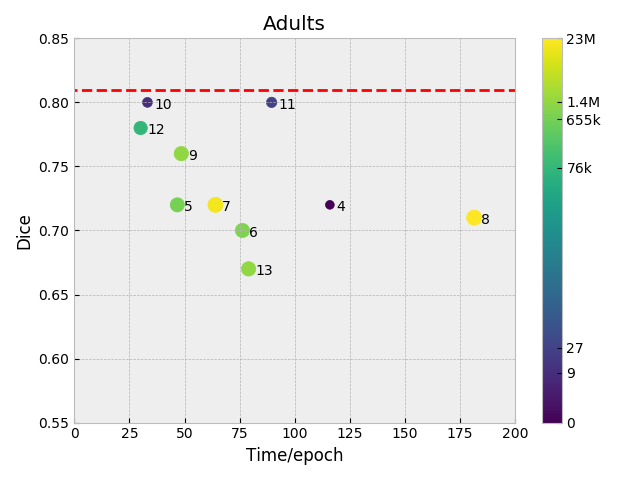
\includegraphics[width=\textwidth]{img/adults}
%   \caption{Dice index on adults}
% \end{subfigure}%
% \begin{subfigure}{.5\textwidth}
%   \centering
%   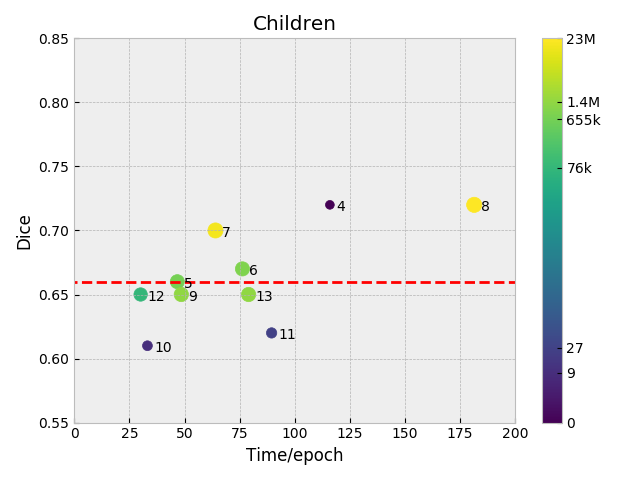
\includegraphics[width=\textwidth]{img/children}
%   \caption{Dice index on children}
% \end{subfigure}
% \caption{Comparing transfer methods. The x axis is the time in seconds taken by one epoch, the y axis is the Dice index. The color represents the number of trainable parameters in a logarithmic scale.}
% \label{fig:tradeoff}
% \end{figure}

%If we do not have access to the source dataset, we have to use a transfer method. Figure~\ref{fig:tradeoff} shows the performance of each transfer strategy compared to the baseline. Fine tuning works really well if we do not care about the performance on the source dataset. Otherwise, two models offering good trade-offs are numbers 9 and 12. Number 9 is surprising as the transfer blocks are residual, and in all other cases where we tried residual connections, it gave worse results.
%Number 12 uses only one transformation layer, therefore adding very few parameters and being fast to train. Surprisingly adding more transformation layers gives worse results as number 13 shows.

%Number 7 and 8 seem appealing on first sight as they give results similar to fine tuning, but at the cost of adding more parameters to the network than it had originally. 

For the transfer methods, the fine-tuning easily beats the children baseline, but does not reach the performance of the joint baseline on either dataset. Moreover, while it does not add any parameter to the network, it takes more time to train than most other transfer methods (this is due to the fact that we have to compute the gradient of every parameter in the network).

Adding fixed convolutional layers did not work. We were able to reach the performance of the fine tuning, but only by adding $3 \times 3 \times 3$ convolutional layers after every downsampling and upsampling layers (line  ``FIxed Convolutions'' in Table~\ref{table:results}). This added 23 millions parameters to the network (it originally had 16 millions) and took longer to train than the fine tuning.

``Geometric Input'' means that we predict the parameters of a geometric transformation before the first layer of the network as described in Section~\ref{ssec:geo_transfo}. It is fast to train and beats the children baseline but fine tuning gives better performance. Likewise for ``Intensity'' only, which means putting an intensity layer at the deepest layer of the U-Net (Section~\ref{ssec:intensity_transfo}).

The best results were obtained by combining the geometric input and learning to predict the parameters of an intensity transformation of the feature maps at the lowest level of the U-Net. This position for the intensity transformation works better than the others. This method adds a small amount of parameters, is fast to train and improve the performance over fine tuning.

%%%%%%%%%%%%%%%%%%%
\subsection{Examining common failures}

\begin{figure}[htb]
  \begin{subfigure}[b]{0.5\linewidth}
    \centering
    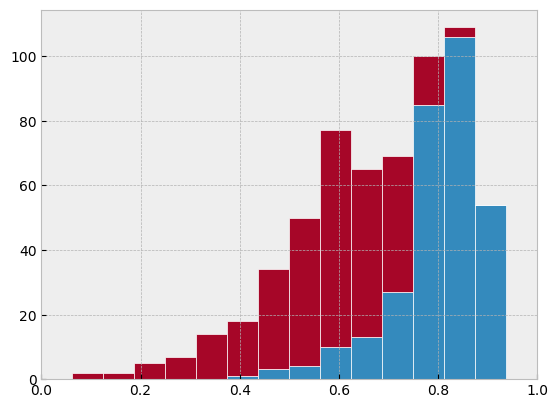
\includegraphics[width=0.95\linewidth]{img_transfer/hist_adults} 
  \end{subfigure}%% 
  \begin{subfigure}[b]{0.5\linewidth}
    \centering
    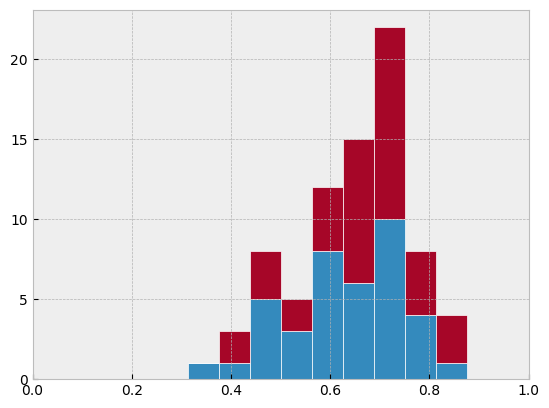
\includegraphics[width=0.95\linewidth]{img_transfer/hist_children} 
  \end{subfigure} 
  \caption[Histogram of Dice coefficient on baseline models]{Histogram of Dice coefficient on baseline models. In red is the adults baseline, blue is the children baseline. Left: Dice coefficient on adults, right: Dice coefficient on children.}
  \label{fig:hist} 
\end{figure}

\begin{figure}[htb]
    \centering
	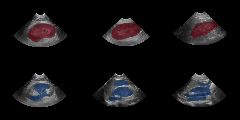
\includegraphics[width=\textwidth]{img_transfer/seg_good_bad}
    \caption[Middle slice of 6 different volumes and a network segmentation superposed on it]{Middle slice of 6 different volumes and a network segmentation superposed on it. The top row shows good segmentations with a Dice index $> 0.90$. The bottom row shows segmentations with a Dice index between $0.60$ and $0.70$. They show the most common mistakes made by the network.}
    \label{fig:mseg}
\end{figure}

Examining in details the results of the different networks, we can observe a few trends. From the histograms of the Dice coefficient in Figure~\ref{fig:hist}, we note that a few of them have a very low Dice index ($< 0.20$). We show some of these images in Figure~\ref{fig:bad_images}. Moreover they are consistently bad for all tested models. All three images are of very low quality, and there are shadows hiding parts of the images. Fortunately, they represent less than $1 \%$ of our dataset.

\begin{figure}[htb]
\centering
\begin{subfigure}{.33\textwidth}
  \centering
  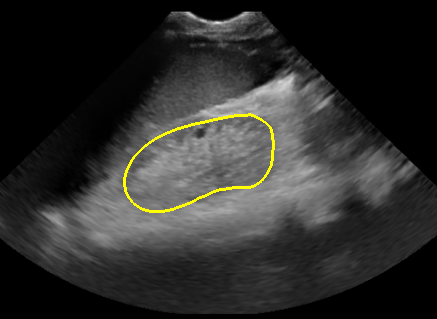
\includegraphics[width=.95\textwidth]{img_transfer/adult_bad}
\end{subfigure}%
\begin{subfigure}{.33\textwidth}
  \centering
  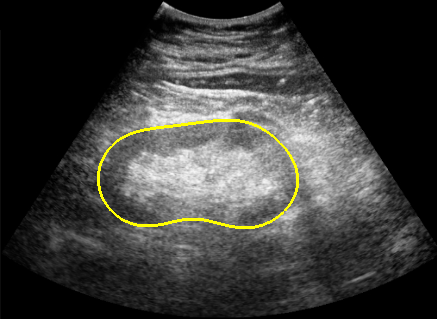
\includegraphics[width=.95\textwidth]{img_transfer/adult_less_bad}
\end{subfigure}
\begin{subfigure}{.33\textwidth}
  \centering
  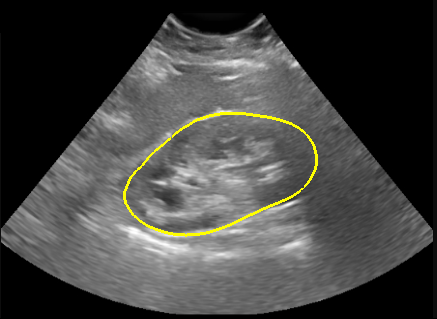
\includegraphics[width=.95\textwidth]{img_transfer/child_less_bad}
\end{subfigure}
\caption{Images on which all models fail to generalize well.}
\label{fig:bad_images}
\end{figure}

Looking at the other images, two kinds of failures were dominant. Either there were multiple connected component in the segmentation or the segmentation were bigger than the ground truth. Some representative samples are shown in Figure~\ref{fig:mseg}. The multiple connected component in the segmentation result from a lack of constraint on the shape of the segmentation. A big segmentation containing the ground truth or a segmentation with multiple connected component can have a high dice value. Adding constraints to the loss could also help to solve some of the common mistakes. Other ways to alleviate the problem would be to smooth the segmentation or to use a shape model, for example using a Conditional Random Field such as in~\textcite{kamnitsas2017MEDIA}.

%%%%%%%%%%%%%%%%%%%%%%%%%%%%%%%%%%
\section{Conclusion}
\label{sec:transfer_conclusion}

We proposed a new transfer method taking advantage of the particularity of the image format of our problem to obtain better results than the more generic fine-tuning. This new method could be applied to other medical imaging problems, with a few caveats. First, if access to the source dataset is possible, joint training on the source and target should be preferred over any transfer method. Secondly, if changes to the structure of the network are impossible (for example if the architecture is hard-coded in released software), our method cannot be used. Finally, it depends on the nature of the differences between the source and target distributions. Our method is efficient in the case of geometric and/or intensity differences, making it well suited for medical imaging problems.
